\chapter{Testrig}
\section{Introduction}
When designing a complex system such as a hybrid vehicle, being continuously be
able to test the system is important to validate that the requirements are met
and to verify the models. To be able to do a full system test, the car has to be
physically run on a track. This can be cumbersome, or in the case of the London
track, impossible at times. Therefore, a test rig is designed and built. The
design process uses the V-model approach with a set of live requirements and
continuous unit and integration testing. The overall goal is to not only be able
to do a faithful simulation of the EcoCar track in London, but to be able to
supply any track (with certain limitations on power and speed demands) to the
test rig and simulations on the car.

\section{Requirements}
The requirements on the test rig are designed to capture the essential demands
on the system. Firstly, the high level User requirements are set. These are set
to capture the problem and to describe the goal of designing the system
~\cite{ibm_req}. The User requirements are then developed into the System
requirements that describe the limitations and demands on the system and its
subsystems.

\section{Car dynamics} \label{sec:cardynamics}
The calculations in this section are in many ways the same as the calculations
given in the previous teams report in Appendix~\ref{app:elba2015}. Though some
of the equations are repetition of what was done last year, they are
done here again with some improvements and more references to make the
derivations of the equations clearer. 

When simulating a track, one needs to know the force exerted by the environment
on the car. A graphical representation of the forces that act on the car is
given in Figure~\ref{fig:testrig_elbadynamics}.
\begin{figure}[H]
    % TODO: Make a better picture!
    \label{fig:testrig_elbadynamics}
    \centering
    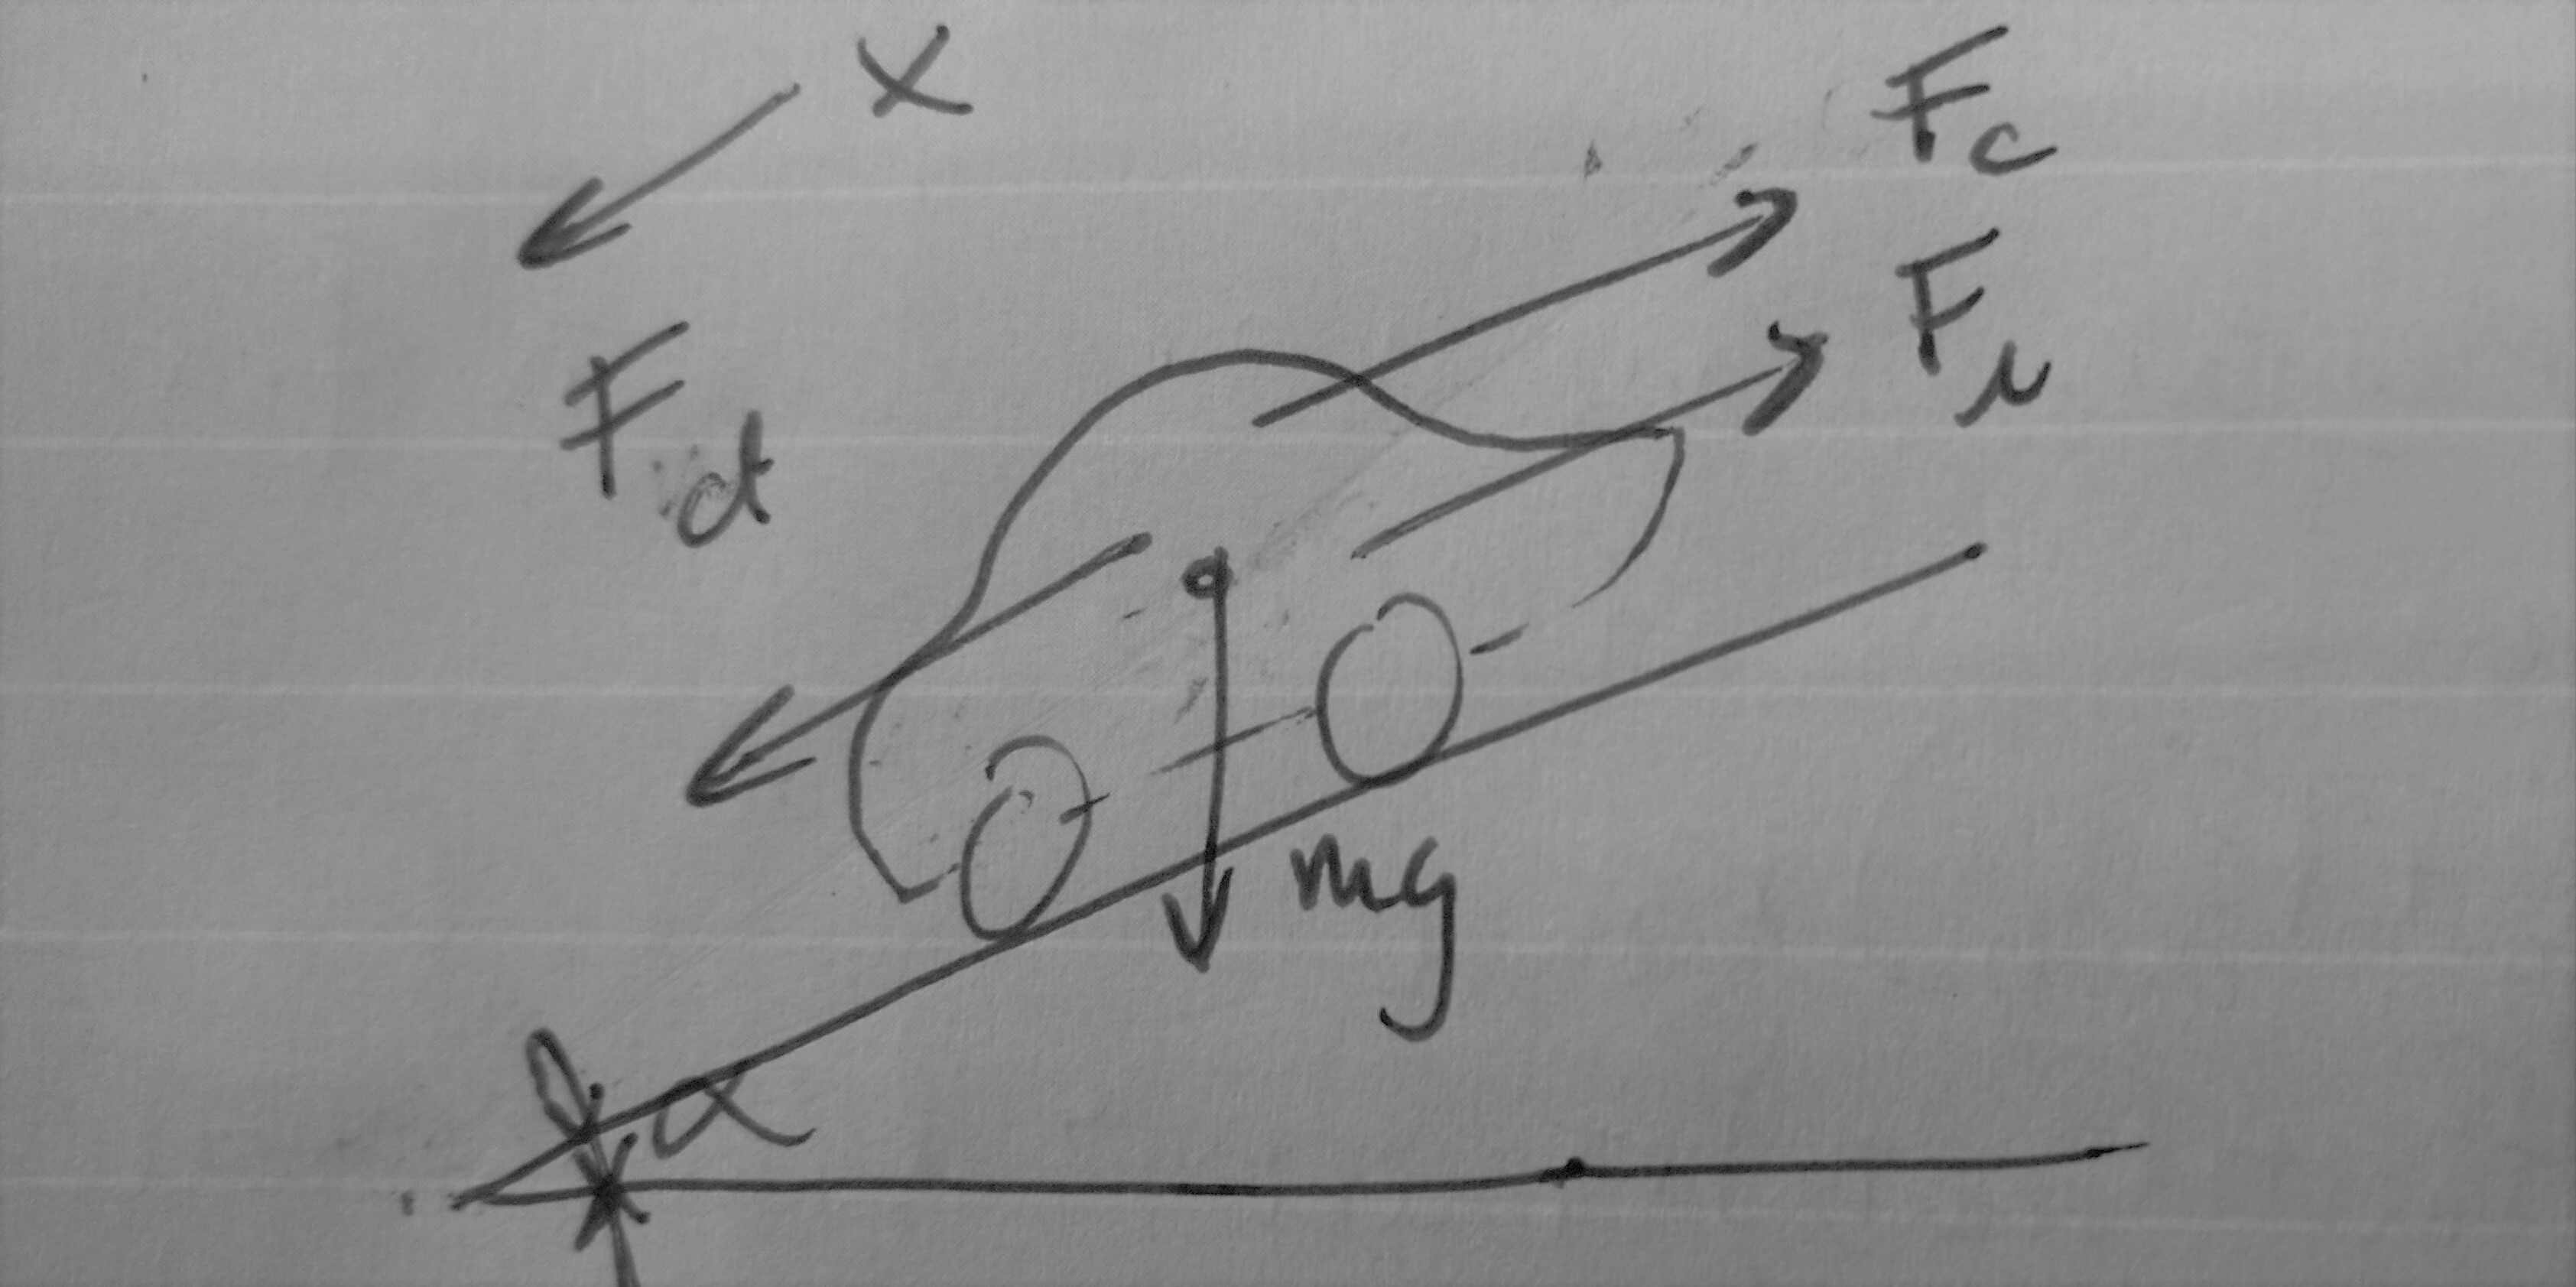
\includegraphics[width=0.5\textwidth]{./img/testrig_elbadynamics.png}
    \caption{Dynamic model of ELBA.}
\end{figure}
The motion equations on the system are 
\begin{equation} \label{eq:testrig_cardynamics}
    m\ddot{x} = F_d + mg\sin{\alpha} - F_c - F_{\mu},
\end{equation}
where $F_d$ is the effective driving force of the car, $m$ is the mass of the
car and $alpha$ is the slope from the horizontal plane. The resistance terms
$F_c$ and $F_{\mu}$ are air and road resistance, respectively. The air drag $D$
around an object can be calculated as \cite{nakayama2002}
\begin{equation} \label{eq:testrig_airdrag}
    D = C_D A \frac{\rho v^2} {2}
\end{equation}
with object velocity $v$, surface area vertical to the movement direction $A$
and air density $\rho$. Most terms in Equation~(\ref{eq:testrig_cardynamics})
are constant throughout a driving instance. Rewriting to
\begin{equation} \label{eq:testrig_csimple}
    C_{tot} = \frac{C_D A \rho} {2}
\end{equation}
yields a simplified equation that only depends on the velocity,
\begin{equation} \label{eq:drag}
    F_D = C_{tot}v^2.
\end{equation}
The total drag coefficient $C_{tot}$ will depend on the vertical area, the density of
air and the drag coefficient $C_D$. The air density is considered to be constant
and is known. The area of Elba can be estimated using simple methods. Finally,
the air drag coefficient $C_D$ is unique to each and every object and is
determined experimentally. For this project, the estimations given for a
passenger car is used. Detailed calculations and values are given in
Appendix~\ref{app:rigdata}. 

% This section is under construction. Need some reference/experiment on how to 
% model rolling friction.
The rolling friction of a car is modeled as a stepfunction, being non-zero at
all velocities that are not zero.

With the air drag, rolling friction and gravity terms known, only two terms of
Equation (\ref{eq:testrig_cardynamics}) are unknown. To fully model the cars
dynamics, the inerta term needs to be modeled. Since the weight of the vehicle
is known, $\ddot{x}$ needs to be derived for an accurate system model.
Knowing the radius of the rollers and the cars wheels, the linear acceleration
can be calculated by measuring the rotational acceleration on the roller. This
is done by an incremental encoder on the roller shaft. Rotational speed is
calculated in the microcontroller and rotational acceleration is derivated from
rotational speed. Using the roller radius, $r_{roller}$, the linear acceleration
is calculated.

Rewriting Equation (\ref{eq:}), (\ref{eq:drag}) and the friction force gives the
desired linear testrig simulation force on the right hand side,
\begin{equation} \label{eq:simulationforce}
    F_d = m\ddot{x} - mg\sin{\alpha} + C_{tot}\dot{x}^2 + F_{\mu}.
\end{equation}

\section{Testrig dynamics}
In order to let the testrig output the correct linear force to the car, the
controller for the testrig need to know the dynamics of te testrig itself. This
is to compensate for internal frictions and inertias. The driveline of the
testrig has two separate steps, the motor and the roller, connected by a chain
gear with gear ratio $n_{chain}$. A prinicple schematic of the testrig from
motor to roller is displayed in Figure~\ref{fig:testrig_testrigdynamics}.
\begin{figure}[H]
    %TODO: Need a better picture!
    \label{fig:testrig_testrigdynamics}
    \centering
    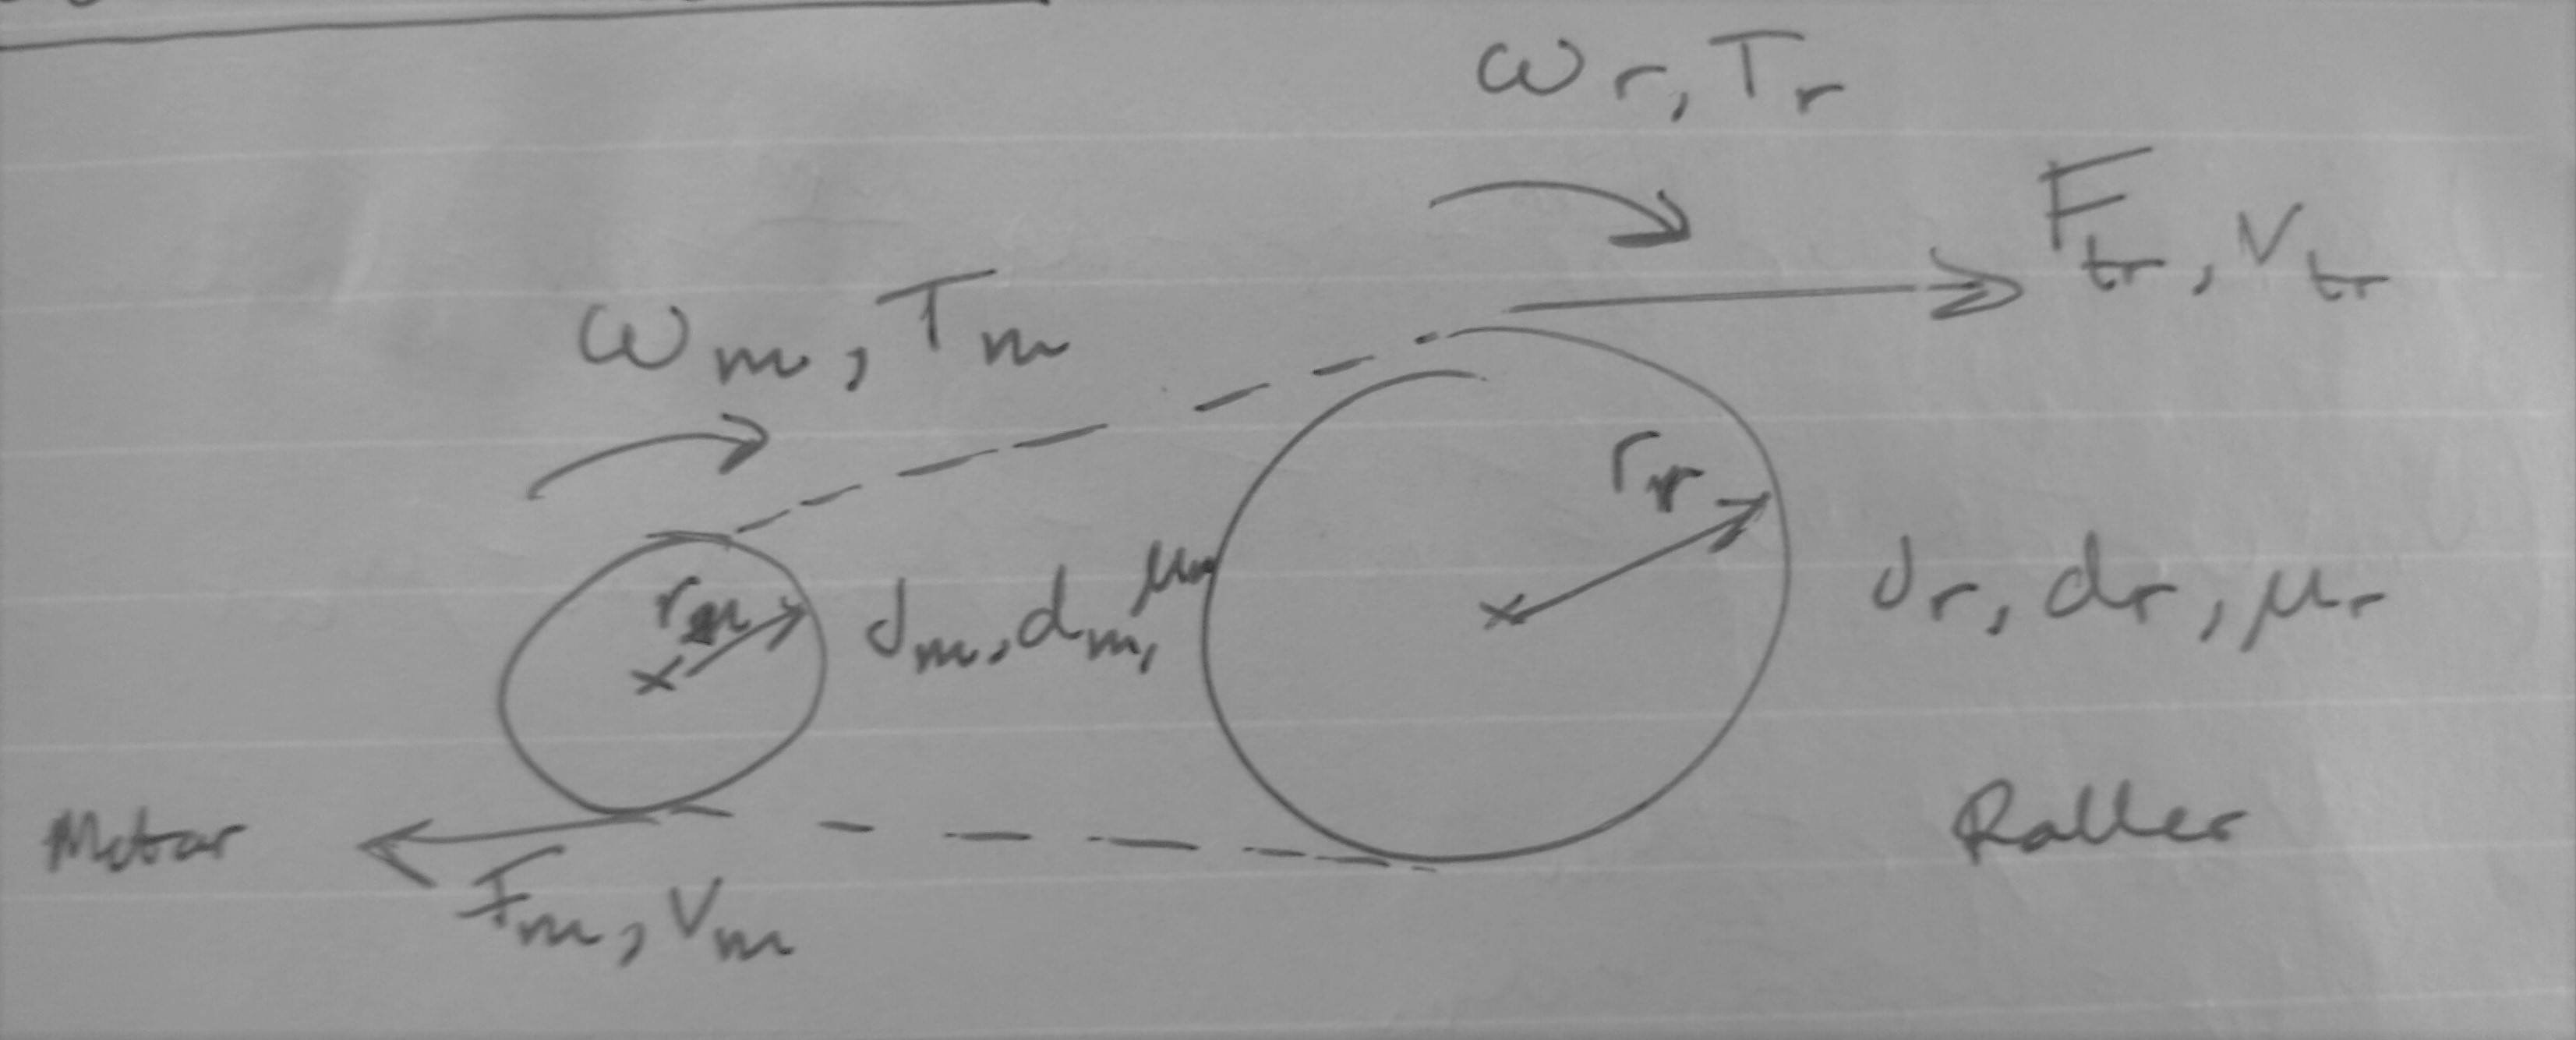
\includegraphics[width=0.9\textwidth]{./img/testrig_testrigdynamics.png}
    \caption{Principle schematic of the testrig from motor to roller.}
\end{figure}
The dynamic equations for the rollers are
\begin{equation} \label{eq:testrig_rollerdynamics}
    J_r \dot{\omega}_r = F_{tr}r_r - d_r \omega_r - \mu_r,
\end{equation}
where $J_r$ is the inertia of the rollers and $\omega_r$ is the rotational velocity
of the roller. The frictional terms are the viscous friction $d_r$ and the
constant friction $\mu_r$ which is modelled by the Karnop model (??). 

Connecting the rollers and the motor is a chain gear. It is modelled as a
generic gear box. A principle drawing of it is given in
Figure~\ref{fig:testrig_chaingear}. 
\begin{figure}[H]
    \label{fig:testrig_chaingear}
    \centering
    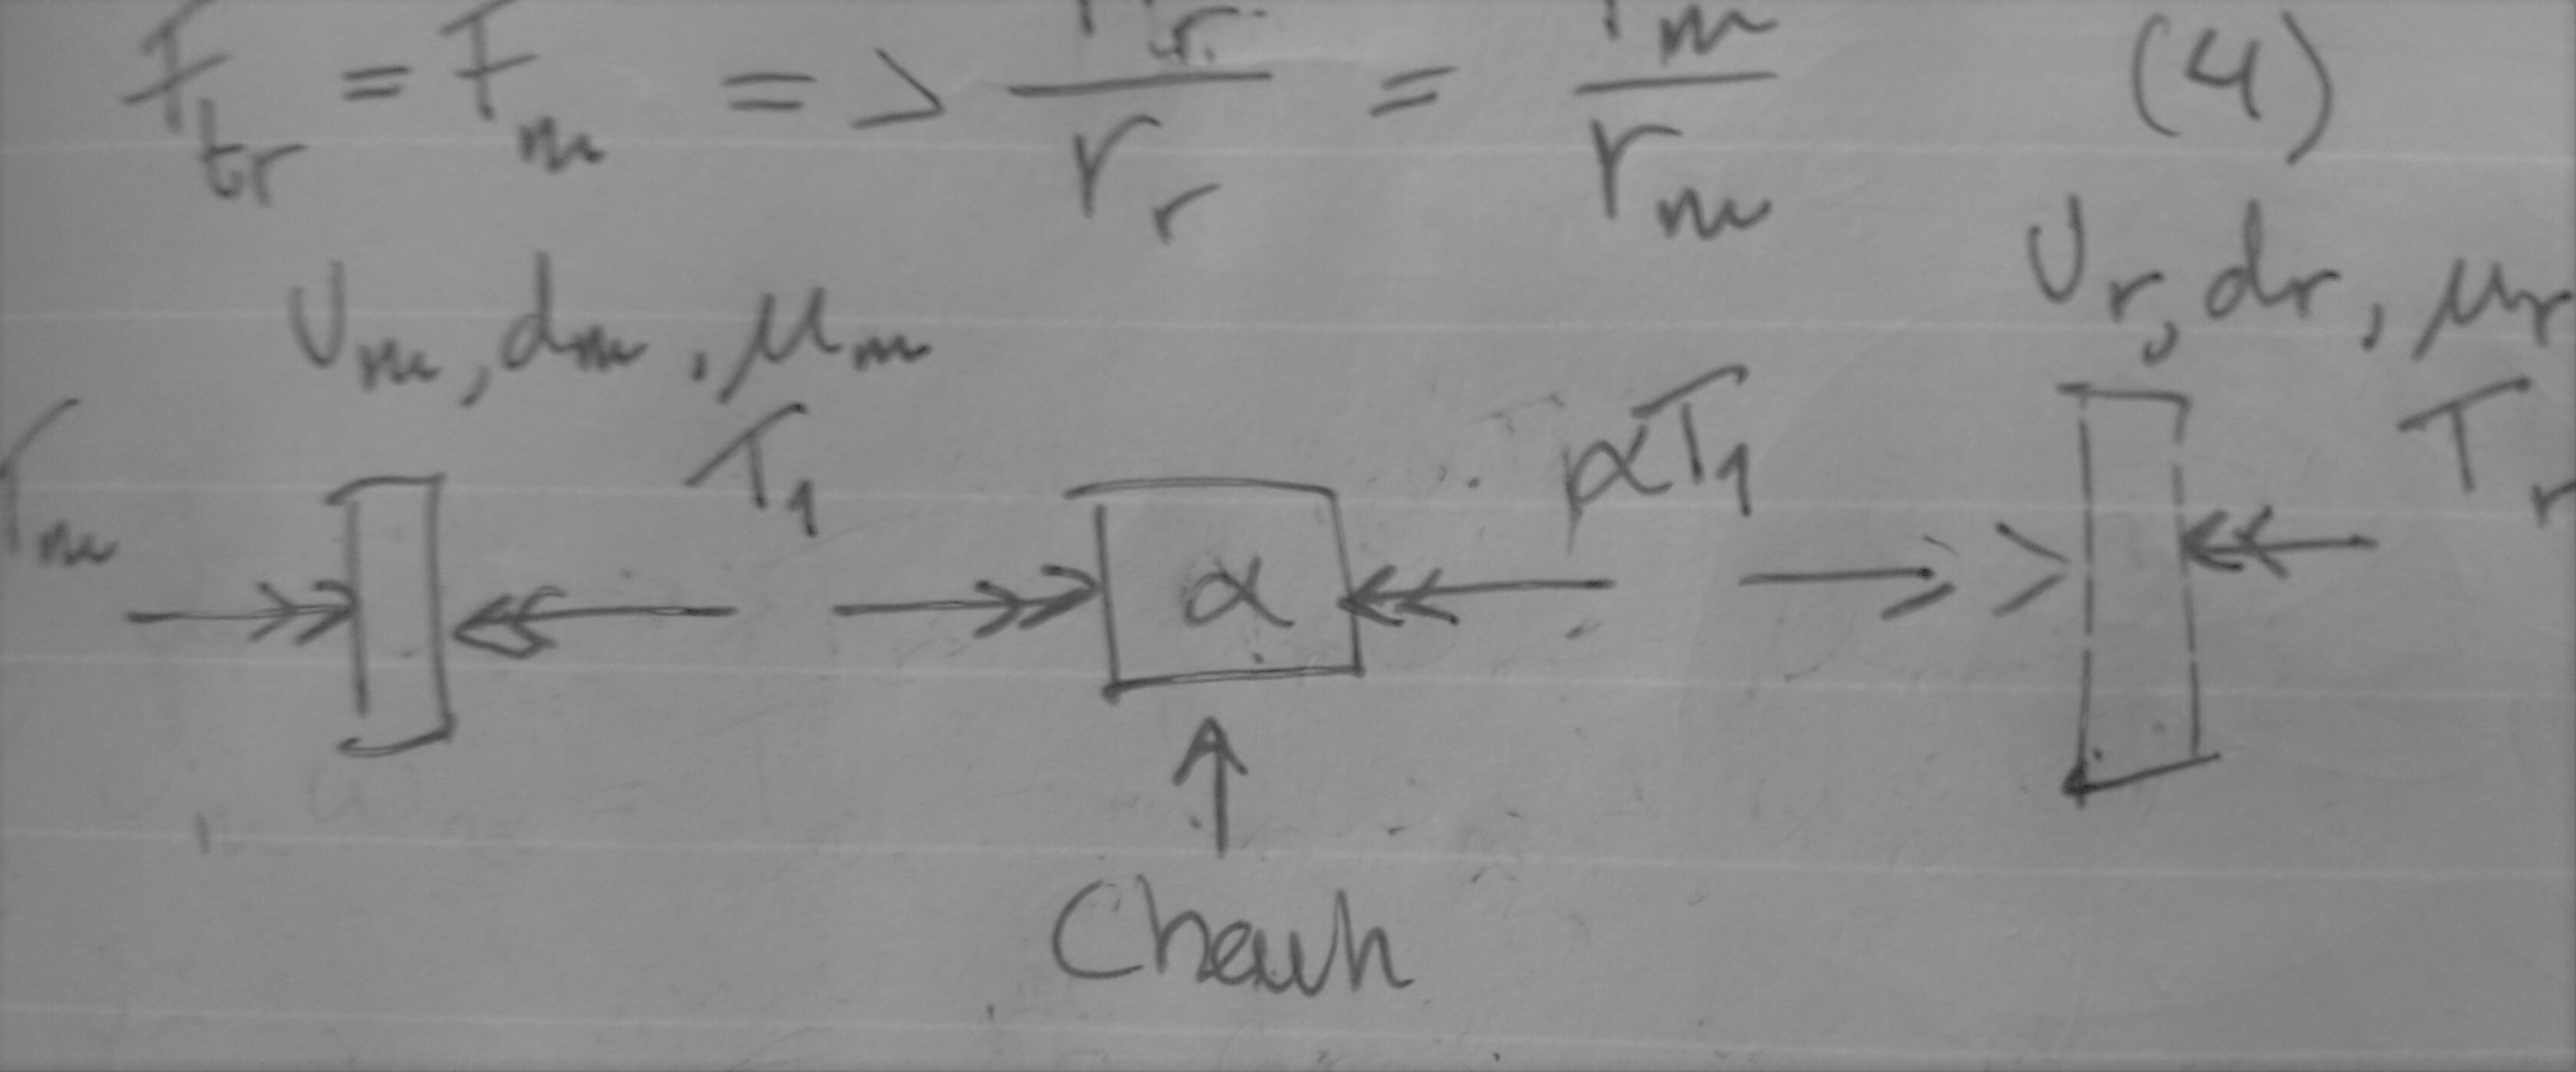
\includegraphics[width=0.9\textwidth]{./img/testrig_chaingear.png}
    \caption{Chaingear modelled as a generic gearbox with no internal friction.}
\end{figure}
This gearbox model has no internal friction.  There is always friction in a
chain gear but it is expected that this friction will be incorporated in the
total system model and the friction free representation is deemed adequate.
Using Equation (\ref{eq:testrig_rollerdynamics}) and (motor model) along with
the gearbox model, the total testrig dynamic model becomes
\begin{equation} \label{eq:testrig_totaldynamics}
    J_{tot} \dot{\omega_m} = T_m + F_tr r_r - d_{tot} \omega_m - \mu_{tot},
\end{equation}
with motor torque $T_m$, simulation force $F_{tr}$ and motor rotational velocity
$\omega_m$. The inertia term is the combined inertia of the motor and
roller,
\begin{equation} \label{eq:totalinertia}
    J_{tot} = J_m + J_r \frac{1} {n^2}.
\end{equation}
The friction terms are combined terms as well, namely
\begin{equation} \label{eq:testrig_totalvfric}
    d_{tot} = d_m + d_r \frac {1} {n}
\end{equation}
and
\begin{equation} \label{eq:testrig_totalfric}
    \mu_{tot} = \mu_m + \mu_r.
\end{equation}



\section{Temp notes}
Modelled negative forces acting on vehicle (gravity, air resistance, friction): 

\begin{figure}[H]
    \label{fig:testrig_negative_forces}
    \centering
    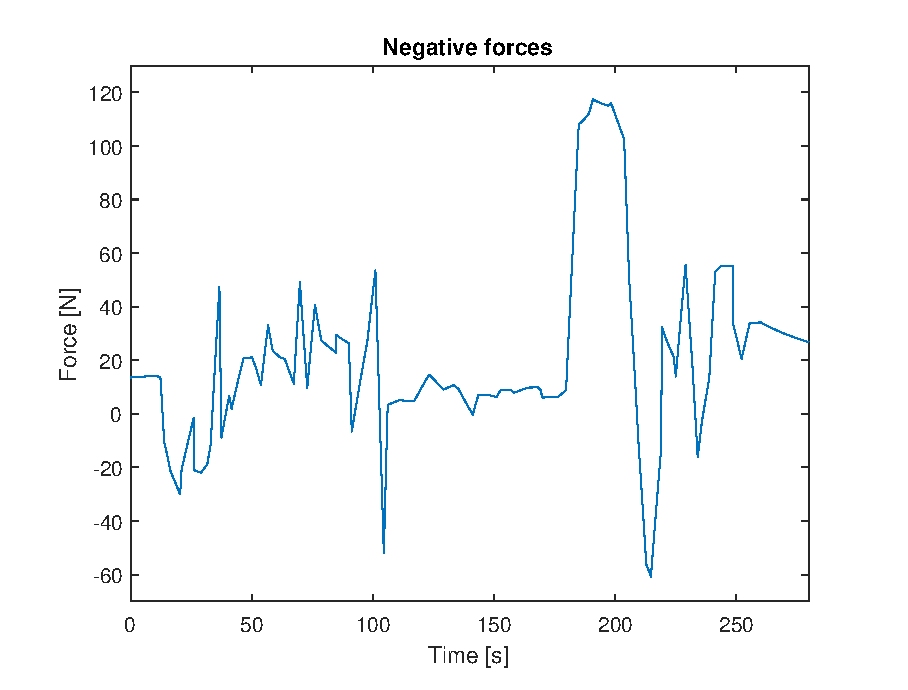
\includegraphics[width=0.5\textwidth]{./img/testrig_negative_forces.eps}
    \caption{Negative forces acting upon Elba in one lap.}
\end{figure}

Torque required on wheel of ELBA:$$T_w = F_n\*r_w$$

Torque required for roller on test rig: $$T_r = \frac{T_w\*r_r}{r_w}$$

Required torque for motor, $T_m$: $$T_m = T_t + J_r\*\ddot{\phi} + d\*\dot{\phi}_m + k\*\phi_m$$

Power required for motor: $$P_m = T_m\*\dot{\phi}_m$$

The inertia $J_r$ for the rollers on the testrig was calculated to be $0.0039$ $kgm^2$

This results in $P_m = 1000$ W

\begin{figure}[H]
    \label{fig:testrig_power_required}
    \centering
    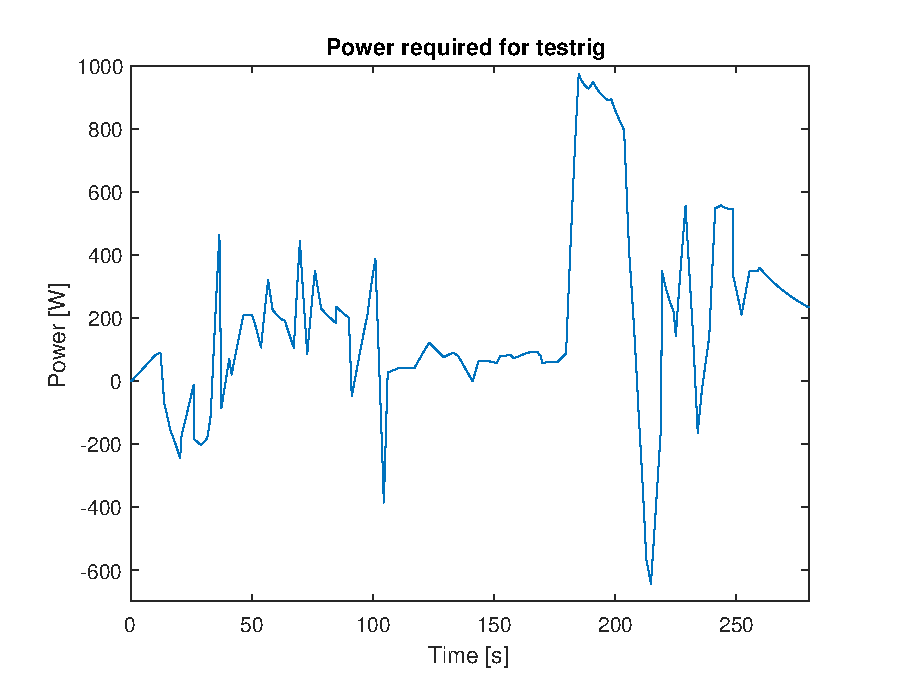
\includegraphics[width=0.5\textwidth]{./img/testrig_power_required.eps}
    \caption{Power required for the motor on the testrig.}
\end{figure}
